%%% PREAMBLE - Do not touch %%%%%%%%%%%%%%%%%%%%%%%%%%%%%%%%%%%%%%%%%%%%%%%%%%%%%%
\documentclass[10pt,twocolumn,letterpaper]{article}
\usepackage[ansinew]{inputenc}
\usepackage[portuges,brazil,english]{babel}
\usepackage{model}
\usepackage{times}
\usepackage{epsfig}
\usepackage{graphicx}
\usepackage{amsmath}
\usepackage{amssymb}
\usepackage{color}
\usepackage[pagebackref=true,breaklinks=true,letterpaper=true,colorlinks,bookmarks=false]{hyperref}

\cvprfinalcopy % *** Uncomment this line for the final submission
\def\httilde{\mbox{\tt\raisebox{-.5ex}{\symbol{126}}}}
\ifcvprfinal\pagestyle{empty}\fi

\newcommand{\CITEONE}[2]{\mbox{#1 \cite{#2}}}
\newcommand{\CITETWO}[3]{\mbox{#1 and #2 \cite{#3}}}
\newcommand{\CITEN}[2]{\mbox{#1 et al. \cite{#2}}}

%%% Report beginning %%%%%%%%%%%%%%%%%%%%%%%%%%%%%%%%%%%%%%%%%%%%%%%%%%%%%%%%%%%%%%
\begin{document}

%%% Title and authors %%%%%%%%%%%%%%%%%%%%%%%%%%%%%%%%%%%%%%%%%%%%%%%%%%%%%%%%%%%%
\title{Predicting revenue in movies}
\author{Vin\'{i}cius Silva \\ email         \href{vinicius.lopes.silva89@gmail.com}{vinicius.lopes.silva89@gmail.com} 
\\ \and
Mario Costa \\ email \href{mariokozta@gmail.com}{mariokozta@gmail.com}
}

%%% Abstract %%%%%%%%%%%%%%%%%%%%%%%%%%%%%%%%%%%%%%%%%%%%%%%%%%%%%%%%%%%%%%%%%%%%%
\maketitle
\begin{abstract}
Predicting the amount of money a movie can make is a valuable tool when deciding if a movie should be made or what should be adjusted for it to be successful. The revenue a movie might have is an important indicator that could be used for detecting the movies faults or qualities. This paper proposes an approach to solve this problem
\end{abstract}

%%% Introduction %%%%%%%%%%%%%%%%%%%%%%%%%%%%%%%%%%%%%%%%%%%%%%%%%%%%%%%%%%%%%%%%%
\section{Introduction}
The movie industry might not be able to properly know when a movie will have a high or low revenue. Of course, it is possible for some members of this industry to have a good feeling for that, but otherwise, it is unknown. Being able to predict how much income a movie will have is a valuable tool before producing a movie. With this information in hand, the studio could know if it will spend too much on the movie or even if it is viable to produce the movie. 

%%% Add section %%%%%%%%%%%%%%%%%%%%%%%%%%%%%%%%%%%%%%%%%%%%%%%%%%%%%%%%%%%%%%%%%%
\section{Problem}
This paper proposes to create a predictive model about how much revenue a given movie can have. In order to do this, the dataset in \cite{dataset} is going to be used. The amount of revenue a movie can have will vary according to the time it has passed after its launch. For this research, we are going to adopt the revenue found in the dataset and validate the predictions using this same dataset.

%%% Add section %%%%%%%%%%%%%%%%%%%%%%%%%%%%%%%%%%%%%%%%%%%%%%%%%%%%%%%%%%%%%%%%%%
\section{Proposed Solution}
A movie revenue could vary based on its opening week, genre, actors and other unknown variables. Since the variables might vary and are not necessarily known, this paper proposes an approach based on clustering algorithms and then running a regression model for each discovered cluster. 

\begin{figure}[h!]
 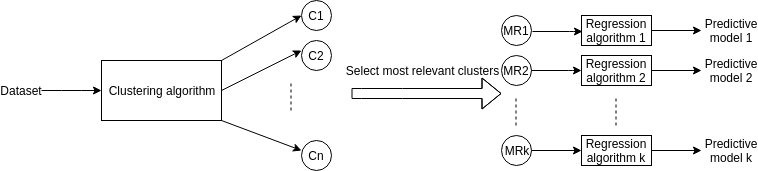
\includegraphics[width=0.99\columnwidth]{pics/methodology.png}
 \caption{Flow describing the approach to predict movies revenue.\label{fig:methodology}}
\end{figure}

The approach illustrated in \ref{fig:methodology} can be described in the following steps:
\begin{enumerate}
  \item Run clustering algorithms in dataset.
  \item Find the most relevant clusters.
  \item Analyze these clusters through the use of regression models.
  \item Find regressive model for each of the relevant clusters.
\end{enumerate}

One could argue that this approach is not optimal, since it could be run a regression model directly in the dataset, however, the accuracy of a prediction model might be increased by taking in consideration other unknown variables that might be related to the prediction of the outcomes \cite{Inf_Front}. By adding clustering, it is possible to analyze what features are more relevant for the revenue of a movie.

It is important to note that this paper does not discard the idea of creating a regression model without the clustering step, but at first the authors prefer to study the impact of the features in the movies and clustering would be helpful in that purpose.


%%% References %%%%%%%%%%%%%%%%%%%%%%%%%%%%%%%%%%%%%%%%%%%%%%%%%%%%%%%%%%%%%%%%%%%
{\small
\bibliographystyle{unsrt}
\bibliography{refs}
}

\end{document}
